\documentclass[12pt]{article}

\usepackage{sbc-template}

\usepackage{graphicx,url}

%\usepackage[brazil]{babel}   
\usepackage[utf8]{inputenc}  

\usepackage{makecell}
     
\sloppy

\title{Análise de Sentimentos utilizando Dicionários Léxicos\\ Uma Revisão Sistemática}

\author{Airton Bordin Junior\inst{1}}


\address{Instituto de Informática -- Universidade Federal de Goiás
  (UFG)\\
  Caixa Postal 131 -- 74690-900 -- Goiânia -- GO -- Brazil
}

\begin{document} 

\maketitle

\begin{abstract}
	abstract here
\end{abstract}

\begin{resumo} 
 	resumo aqui
\end{resumo}


\section{Introdução}
A Mineração de Opiniões, também chamada de Análise de Opiniões ou Análise de Sentimentos, é uma linha de pesquisa abrangente e que vem sendo tema de diversos trabalhos nos últimos anos. Como observado em \cite{liu2010multifaceted}, esse crescente interesse sobre o assunto ocorre principalmente devido ao aumento no número de usuários de Internet e o consequente crescimento da produção de conteúdo independente na rede, como opiniões, avaliações, entre outros. 

Essa área de estudo tem como principal desafio a Análise de Opiniões, descritas em linguagem natural, para a identificação da polaridade implícita ou explícita no texto. Essa polaridade é, na maior parte das vezes, identificada como uma escala de pontuação de sua característica positiva, negativa ou neutra.

Uma das principais técnicas para aumentar a acurácia a Análise de Sentimentos é a utilização de Dicionários de Dados. Esses dicionários contêm palavras previamente avaliadas por especialistas humanos, principalmente quanto à sua polaridade. Neste contexto, esse conjunto de palavras, juntamente com suas polaridades, é chamado de Dicionário Léxico ou Dicionário de Sentimentos. 

Porém, é evidente a limitação inerente à estratégia de utilização do Dicionário Léxico - a própria lista de palavras disponíveis. Esse fato muitas vezes limita a realização de uma análise mais profunda sobre determinado contexto. Nesse sentido, um dos principais desafios na área de Mineração de Opiniões é a criação e ampliação do Dicionário Léxico de forma automatizada, tema central do presente trabalho. Grande parte desses dicionários são construídos de forma manual, fato que caracteriza uma limitação óbvia para a maior parte dos contextos e domínios, como observado em \cite{duwairi2015detecting}. 

Consciente dessa limitação, a ideia principal do presente trabalho é a criação de um processo automatizado de expansão de Dicionário Léxico, sensível a domínios específicos, fazendo uso de técnicas de algoritmos bioinspirados da classe de Computação Evolucionária, mais precisamente Programação Evolucionária. Resumidamente essa classe de algoritmos busca reproduzir processos naturais de evolução, com conceitos de sobrevivência, mutação, entre outros. Esse processo fará a adequação das polaridades das palavras contidas no dicionário de forma a maximizar a corretude das avaliações. Para avaliar a taxa de erro de cada solução parcial gerada, serão utilizados conjuntos conhecidos de documentos previamente avaliados por especialistas humanos, de forma a compará-los com a solução gerada pelo sistema. Para a avaliação, sistemas de classificação de sentimentos disponíveis serão utilizados.

Devido à característica intrínseca do próprio problema, serão utilizadas na pesquisa bases de textos em inglês. Ao mesmo tempo, muitas técnicas utilizadas durante o trabalho também poderão ser utilizadas para resolver problemas em português, com as devidas alterações. 

Espera-se que esse processo, bem como os Dicionários Léxicos por ele gerado, possam ser utilizados como entrada de processos de avaliação em diversas áreas de Mineração de Opiniões como, por exemplo, Análise de Sentimentos em redes sociais. Algumas dessas pesquisas são realizadas na própria instituição, apoiando, assim, o trabalho de outros pesquisadores. Além disso, devido ao caráter automatizado dessa solução proposta, o mesmo processo poderá ser utilizado, avaliado e melhorado para outras situações, contextos e idiomas.

Por fim, a pesquisa e a utilização de diversas técnicas de PNL e expansão automatizada de Dicionário Léxico poderão servir como um \emph{benchmark} dos principais métodos e classificadores, auxiliando na escolha de ferramentas e abordagens para trabalhos futuros em contextos específicos.

Para apoiar a clareza e desenvolvimento da proposta, o presente documento está estruturado da seguinte forma: o capítulo \ref{sec:desc} tratará da descrição do problema, principais limitações e dificuldades no contexto de Análise de Sentimentos. O capítulo \ref{sec:obj} tratará dos objetivos gerais e específicos. A revisão bibliográfica, apresentada no capítulo \ref{sec:bibl}, tem por objetivo criar o embasamento teórico para apoiar nas soluções propostas, apresentando o estado da arte sobre o assunto, bem como a definição de conceitos fundamentais. O capítulo \ref{sec:impact} apresenta o impacto científico da solução e suas possíveis contribuções para a área. A metodologia, descrita no capítulo \ref{sec:met}, descreve a forma como serão desenvolvidas cada uma das etapas do processo, seguida do capítulo com uma previsão de cronograma do trabalho. Resultados esperados são descritos no capítulo \ref{sec:result}, seguidos da identificação dos colaboradores e participantes do projeto e, por fim, as referências bibliográficas utilizadas na proposta.

\section{Título da seção} \label{sec:firstpage}


\section{Estratégia de Pesquisa}
A Revisão Sistemática da Literatura fornece uma forma estruturada, objetiva e reprodutível de identificar, avaliar e interpretar trabalhos relevantes em uma determinada área de conhecimento. A análise desses trabalhos apoia a resoluções das questões de pesquisa, que devem ser respondidas pelo projeto \cite{Kitchenham2004}.

A definição das questões da pesquisa é uma parte crítica da Revisão Sistemática. Essas mesmas questões são utilizadas de forma a orientar a estratégia de busca e palavras-chave dos artigos nas bases de dados escolhidas.

As questões norteiam, também, os dados e informações que serão relevantes e extraídos dos trabalhos selecionados. Para este trabalho, as questões de pesquisa são as seguintes:

\begin{itemize}
	\item{Quais as principais técnicas empregadas na criação e expansão de Dicionários Léxicos?}
	\item{Estratégias Evolutivas estão sendo utilizadas no contexto de criação e expansão de Dicionários Léxicos?}
	\item{Como a diferença de contexto e domínio vem sendo tratada no contexto de Análise de Sentimentos?}
	\item{Que métricas estão sendo utilizadas para avaliar a qualidade dos algoritmos de criação e expansão de Dicionários Léxicos?}
\end{itemize}

Para a elaboração desta Revisão Sistemática, foram realizadas buscas nas seguintes bases de dados: \emph{Science Direct}, \emph{IEEEXplore}, \emph{ACM Digital Library}, \emph{Research Gate}, \emph{Semantic Scholar}. Essas buscas tem por objetivo coletar os trabalhos primários sobre o tema proposto para a identificação do estado obre o assunto. 

Alguns critérios de seleção dos trabalhos devem ser adotados de forma a realizar a filtragem dos artigos mais relevantes. Para esta revisão, consideramos somente pesquisas realizadas a partir do ano 2000 e que foram publicadas no idioma inglês. Para o presente trabalho, consideramos apenas os artigos disponíveis gratuitamente. A tabela \ref{tab:tab_bases} apresenta as bases de dados utilizadas e os critérios básicos de filtragem.


\begin{table}[ht]
\centering
\begin{tabular}{| c | c | c | c |}
\hline
\textbf{Base de dados} & \textbf{Anos cobertos na busca} & \textbf{Idioma} \\
\hline
\makecell{\emph{Science Direct} \\ http://www.sciencedirect.com/} & 2000 até 2017 & Inglês \\
\hline
\makecell{\emph{IEEEXplore} \\ http://ieeexplore.ieee.org/} & 2000 até 2017 & Inglês \\
\hline
\makecell{\emph{ACM Digital Library} \\http://dl.acm.org/} & 2000 até 2017 & Inglês \\
\hline
\makecell{\emph{Research Gate} \\ https://www.researchgate.net/} & 2000 até 2017 & Inglês \\
\hline
\makecell{\emph{Semantic Scholar} \\ https://www.semanticscholar.org/} & 2000 até 2017 & Inglês \\
\hline

\end{tabular}
\caption{Relação de bases de dados consultadas}
\label{tab:tab_bases}
\end{table}


Baseando-se nas questões de pesquisa demonstradas, foram formuladas palavras-chave para orientar a criação de \emph{strings} de busca nas ferramentas disponibilizadas pelas bases de dados. As palavras escolhidas para o conjunto foram:

\begin{itemize}
	\item{Sentiment Analysis;}
	\item{Opinion Mining;}
	\item{Lexicon Expansion;}
	\item{Genetic Algorithms;}
	\item{Genetic Programming;}
	\item{Semantic Orientation.}
\end{itemize}

Essas palavras-chave representam os principais tópicos da pesquisa, auxiliando na busca e escolha de trabalhos relevantes ao tema. De posse dessas palavras, foram criadas as chaves de busca para a seleção dos artigos. Cada uma das bases de dados apresentadas na tabela \ref{tab:tab_bases} fornece uma ferramenta \emph{online} avançada de busca. Há algumas diferenças entre elas, de forma que foi necessário adequar a \emph{string} para cada uma, conforme apresentado na tabela \ref{tab:tab_palchaves}


\begin{table}[h]
\centering
\begin{tabular}{| c | c |}
\hline
\textbf{\emph{String} de busca} & \textbf{Base de dados} \\
\hline
\makecell{pub-date \textgreater 1999 and (Sentiment Analysis OR Opinion Mining)\\ AND (Lexicon Expansion) AND\\ (Genetic Programming OR Genetic Algorithm) \\ AND (Semantic Orientation)[All Sources(Computer Science)]} & \emph{Science Direct} \\
\hline
\makecell{pub-date \textgreater 1999 and (Sentiment Analysis OR Opinion Mining)\\ AND (Lexicon Expansion OR Lexicon) \\ AND (Semantic Orientation)[All Sources(Computer Science)]} & \emph{IEEEXplore} \\
\hline
\makecell{((Sentiment Analysis OR Opinion Mining)\\ AND (Lexicon Expansion OR Lexicon) \\ AND (Semantic Orientation))  and refined by Year: 2000-2017} & \emph{ACM Digital Library} \\
\hline
\makecell{"query": { (+Sentiment +Analysis Lexicon Genetic Algorithm) } \\ "filter": {"publicationYear":{ "gte":2000 }}} & \emph{Research Gate} \\
\hline
\end{tabular}
\caption{Detalhamento das palavras chave da busca e respectivo idioma}
\label{tab:tab_palchaves}
\end{table}

Após a aplicação das buscas nas respectivas bases, foi realizada uma segunda filtragem dos dados, de forma a selecionar trabalhos relevantes às questões de pesquisa. Essa filtragem foi feita por meio da letura dos resumos dos artigos, buscando identificar os trabalhos relevantes ao propósito da Revisão Sistemática. 

\section{Sections and Paragraphs}

\subsection{Subsections}

\section{Figures and Captions}\label{sec:figs}


Figure and table captions should be centered if less than one line
(Figure~\ref{fig:exampleFig1}), otherwise justified and indented by 0.8cm on
both margins, as shown in Figure~\ref{fig:exampleFig2}. The caption font must
be Helvetica, 10 point, boldface, with 6 points of space before and after each
caption.

\begin{figure}[ht]
\centering
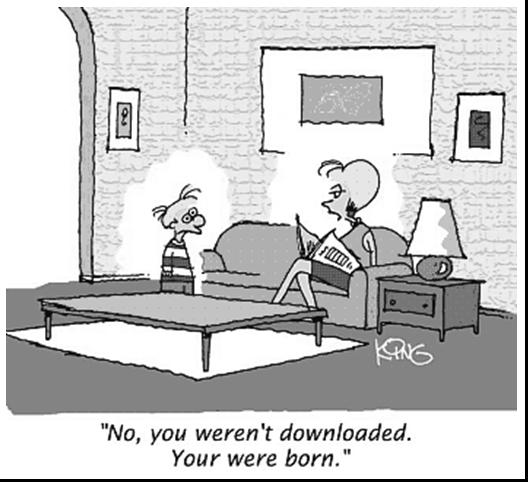
\includegraphics[width=.5\textwidth]{fig1.jpg}
\caption{A typical figure}
\label{fig:exampleFig1}
\end{figure}

\begin{figure}[ht]
\centering
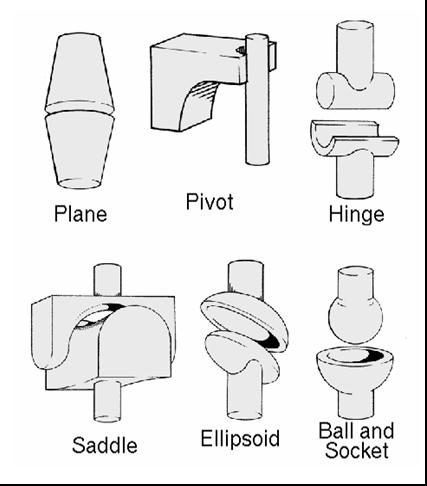
\includegraphics[width=.3\textwidth]{fig2.jpg}
\caption{This figure is an example of a figure caption taking more than one
  line and justified considering margins mentioned in Section~\ref{sec:figs}.}
\label{fig:exampleFig2}
\end{figure}

In tables, try to avoid the use of colored or shaded backgrounds, and avoid
thick, doubled, or unnecessary framing lines. When reporting empirical data,
do not use more decimal digits than warranted by their precision and
reproducibility. Table caption must be placed before the table (see Table 1)
and the font used must also be Helvetica, 10 point, boldface, with 6 points of
space before and after each caption.

\begin{table}[ht]
\centering
\caption{Variables to be considered on the evaluation of interaction
  techniques}
\label{tab:exTable1}
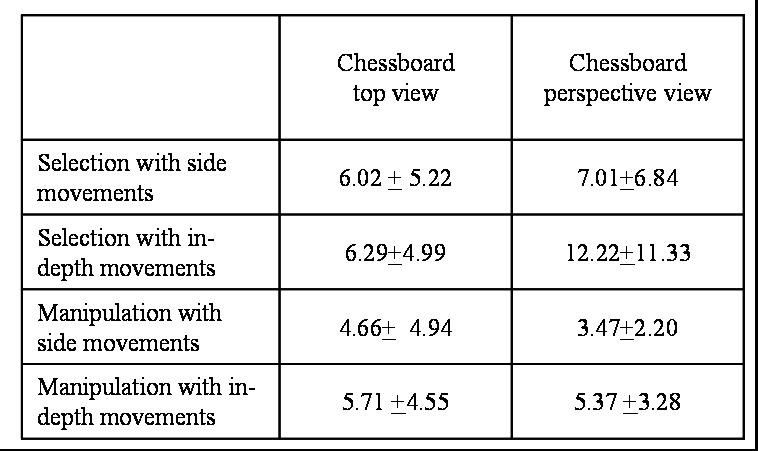
\includegraphics[width=.7\textwidth]{table.jpg}
\end{table}

\section{Images}

All images and illustrations should be in black-and-white, or gray tones,
excepting for the papers that will be electronically available (on CD-ROMs,
internet, etc.). The image resolution on paper should be about 600 dpi for
black-and-white images, and 150-300 dpi for grayscale images.  Do not include
images with excessive resolution, as they may take hours to print, without any
visible difference in the result. 

\section{References}

Bibliographic references must be unambiguous and uniform.  We recommend giving
the author names references in brackets, e.g. \cite{knuth:84},
\cite{boulic:91}, and \cite{smith:99}.

The references must be listed using 12 point font size, with 6 points of space
before each reference. The first line of each reference should not be
indented, while the subsequent should be indented by 0.5 cm.

\bibliographystyle{sbc}
\bibliography{sbc-template}

\end{document}
